% xform-digraph.tex

\documentclass[tikz]{standalone}
\usetikzlibrary{shapes, positioning, arrows.meta, calc, intersections, backgrounds, fit}

% default horizontal/vertical distance
\def\hdist{1.3}
\def\vdist{1.3}
\tikzset{node distance = \vdist and \hdist}

\newcommand{\state}[3]{% #1: name; #2: position; #3: label
  \node (#1) [circle, inner sep = 1pt, minimum size = 5mm, align = center, draw, #2, font = \scriptsize] {#3};
}

\newcommand{\trans}[5]{% #1: start state; #2: end state; #3: label position; #4: label; #5: style
  \draw[>=Stealth, ->, #5] (#1) to node [rectangle, draw, #3 = 2pt, sloped, inner sep = 1pt, font = \tiny] (#1#2) {#4} (#2);
}

\begin{document}
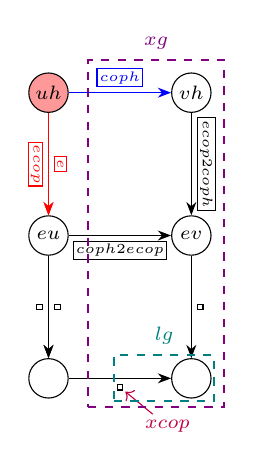
\begin{tikzpicture}
  \state{uh}{fill = red!40}{$uh$}
  \state{eu}{below = of uh}{$eu$}
  \state{vh}{right = of uh}{$vh$}
  \state{ev}{right = of eu}{$ev$}

  \trans{uh}{eu}{below}{$ecop$}{red}
  \trans{uh}{eu}{above}{$e$}{red}
  \trans{uh}{vh}{above}{$coph$}{blue}
  \trans{eu}{ev}{below}{$coph2ecop$}{}
  \trans{vh}{ev}{above}{$ecop2coph$}{}

  \state{1}{below = of eu}{}
  \state{2}{right = of 1}{}
  \trans{eu}{1}{above}{}{}
  \trans{eu}{1}{below}{}{}
  \trans{ev}{2}{above}{}{}
  \trans{1}{2}{below}{}{}

  \node (xcop) [purple, font = \scriptsize, below right = 0.3cm and 0.2cm of 12, inner sep = 2pt] {$xcop$};
  \draw[->, shorten >= 1pt, purple] (xcop) to (12);

  \node (xg) [thick, dashed, violet, font = \scriptsize, draw, inner sep = 3pt, fit = (uhvh) (2) (vhev), rectangle, label = {above: \textcolor{violet}{\scriptsize $xg$}}] {};

  \node (lg) [thick, dashed, teal, font = \scriptsize, draw, inner sep = 1pt, fit = (12) (2), rectangle, label = {above: \textcolor{teal}{\scriptsize $lg$}}] {};
\end{tikzpicture}
\end{document}
